\documentclass[../report.tex]{subfiles}

%\usepackage{import}
%\usepackage[left=2cm, right=2cm, top=2.5cm]{geometry}
%\usepackage{algorithm}
%\usepackage{algorithmic}
%\usepackage[absolute,overlay]{textpos}
%\usepackage{graphicx}
%\usepackage[export]{adjustbox}
%\usepackage{caption}
%\usepackage{subcaption}


\begin{document}


The purpose of the algorithm is to get the cost of a path generated randomly from a set of node $S=\{0,...,n\}$, starting from node 0, with each node visited exactly once. The cost is the sum of the distance $d_{ij}$ between two successive nodes i and j. The distance for nodes that are not connected is set to -1.
\newline{} 
For a subset $S'\subseteq S$ of nodes not yet visited, starting from node j, we compute a probability distribution $P_{k}$, $k \in S'-\{j\}$, for the next possible nodes k based on the distance $d_{jk}$ such that the lower, the higher the probability. From the distribution P, the cumulative distribution P' is constructed using increasing probabilities $P_{k}$.  A random number r between 0 and 1 is picked from a uniform distribution. For r such that $P'_{k-1}< r <P'_{k}$, the node k is picked.


\[ sum = \sum_{k \in S'-\{j\}} d_{jk}, \quad {where} \quad d_{jk}!=-1 \]   
\[ P_{k} = (sum - d_{jk})/(sum*(n-1)), \quad \textit{where n number of node in S'-\{j\} connected to node j}\]
The division by (n-1) allows normalization so that $\sum_{k} P_{k}=1$,

\begin{figure}[ht]
\centering
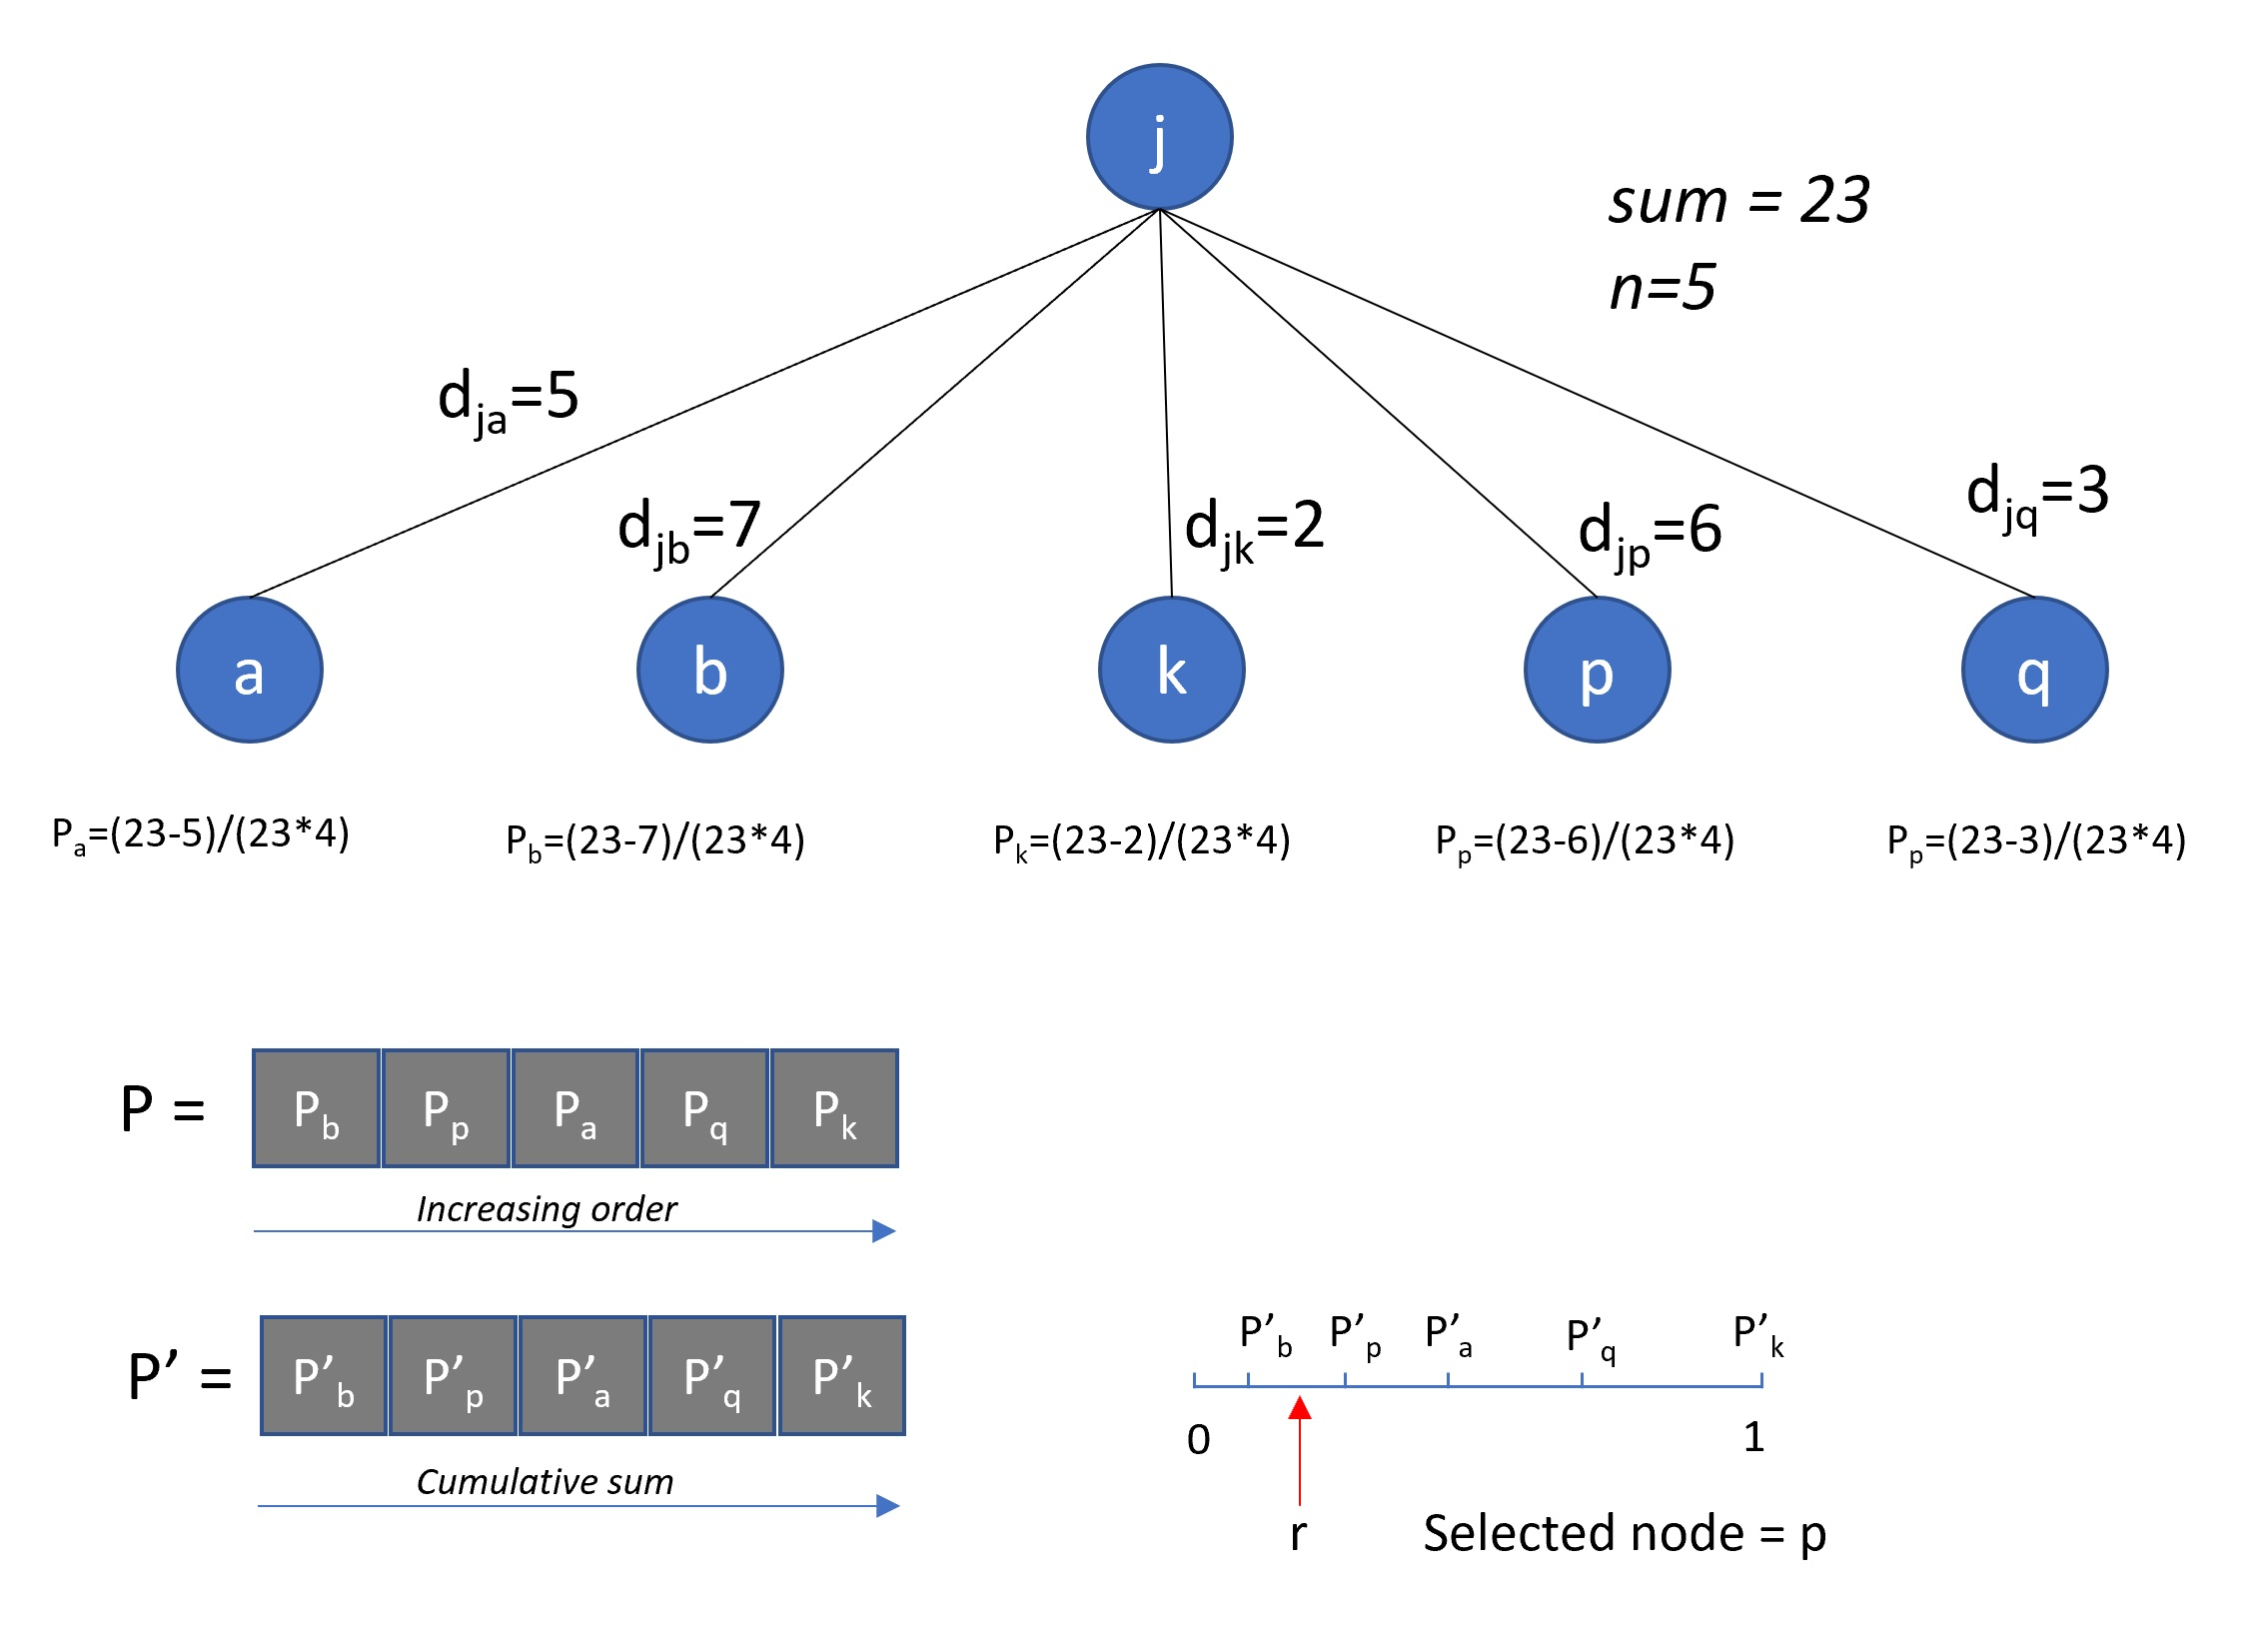
\includegraphics[width=11cm]{../Images/random_algo.jpg}
\caption{Example of node selection \label{overflow}}
\end{figure}

\begin{subsection}{Pseudo code}\hfill

\begin{center}
	\colorbox[gray]{0.95}{
	\begin{minipage}{0.85\textwidth}
\begin{algorithm}[H]
\caption{Randomized Algorithm}
\begin{algorithmic} 
\REQUIRE{  }
   \STATE $d[nbNode][nbNode]$
   \STATE $S=\{1,...,n\}$
\ENSURE {}
\STATE sourcenode := 0
\STATE S' := S
\STATE path := []
\STATE $cost = 0$
\WHILE {$|S'|>1$}
   \STATE sum := 0
   \STATE nbnode := 0
   \FOR {node in S'-\{sourcenode\} with d[sourcenode][node] != -1}
      \STATE sum = sum + d[sourcenode][node]
      \STATE nbnode= nbnode + 1
   \ENDFOR   
   \FOR {k in S'-\{sourcenode\} with d[sourcenode][node] != -1}
      \STATE $P(k) = (sum - d[sourcenode][k])/sum/(nbnode-1)$
   \ENDFOR
   \STATE sort(P)
   \STATE P' := cumulative sum of elements of P
   \STATE r := random(0,1)
   \STATE search k s.t. $P(k-1)<r<P(k)$
   \STATE $cost := cost + d[sourcenode][k]$
   \STATE add k to path
   \STATE remove k from S'
   \STATE $startnode := k$   
\ENDWHILE
\STATE $cost := cost + d[startnode][0]$
\RETURN $cost$, $path$
\end{algorithmic}
\end{algorithm}
\end{minipage}}
\end{center}
\end{subsection}

\begin{subsection}{Complexity}
The algorithm is proceeding from top to down. For each node source (n loops) we compute the probability table of the possible next nodes using operations of the order $O(1)$. The table is sorted in increasing order using Python sort function whose complexity is $O(n log n$). The search of the node whose probability matches the random number is O(log n) using divide and conquer algorithm.
Consequently, the time complexity for the proposed version of randomized algorithm is $O(n^2 log n)$.
For each source node, we compute a probability table of at most n elements. The space complexity is O(n).
\end{subsection}

\begin{subsection}{Performances}


\begin{figure}[H]
\centering
\begin{subfigure}{.5\textwidth}
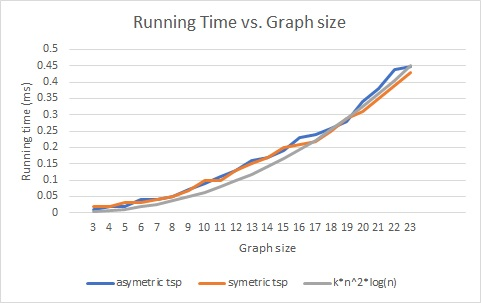
\includegraphics[height=5cm,valign=t]{../Images/perf_random_graphsize.jpg}
\caption{Example of node selection \label{fig:randomgraphsize}}
\end{subfigure}%
\begin{subfigure}{.5\textwidth}
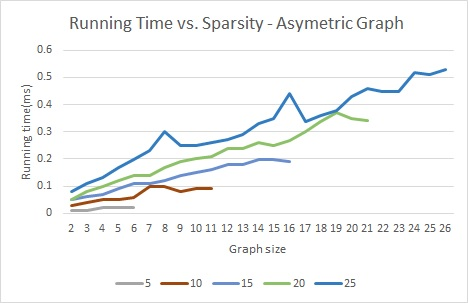
\includegraphics[height=5cm,valign=t]{../Images/perf_random_sparsity.jpg}
\caption{Example of node selection \label{fig:randomsparsity}}
\end{subfigure}%
\caption{Example of node selection \label{fig:randomperf}}
\end{figure}

The algorithm is tested on a set of problems generated randomly with different city numbers and different sparsity.
The algorithm is tested on a set of problems generated randomly with different city numbers and different sparsity.
Figure ~\ref{fig:randomgraphsize} shows the evolution of the algorithm running time with the number of cities. We can observe that the curves for symetric and asymetric problems follow the theoritical complexity of $O(n^2 log n)$. \\
Figure ~\ref{fig:randomsparsity}shows the evolution of the algorithm running time with the number of cities. We can observe that the curves for symetric and asymetric problems fo.



The algorithm is tested on a set of problems from the TSLIB.
The alg

\end{subsection}
\end{document}


